% ======================================================================
% Somnus Sovereign Systems — Canonical Whitepaper Template
%
% This template is designed to give research and doctrine papers a clean,
% retro‑technical appearance reminiscent of late‑1970s and early‑1980s
% computer science literature.  Body text is strictly monochrome – the
% only colour permitted is inside code listings, diagrams, and plots.
% A "Prolegomenon" section replaces the traditional abstract to set the
% philosophical context before technical sections.  Authors can fill in
% the macros below to customise the metadata for each paper.  To build
% a cover page for the same paper, use the accompanying
% ``somnus_cover_page.tex`` template.

\documentclass[11pt,letterpaper]{article}

% ----------------------------------------------------------------------
% Encoding and typography
\usepackage[utf8]{inputenc}
\usepackage[T1]{fontenc}
\usepackage[margin=1.25in]{geometry}  % generous margins evoke the typewriter era
\usepackage{microtype}
\usepackage{newtxtext,newtxmath}  % serif text with matching mathematics
\usepackage{setspace}
\setstretch{1.1}

% ----------------------------------------------------------------------
% Graphics and drawing
\usepackage{graphicx}
\usepackage{tikz}
\usetikzlibrary{arrows.meta,calc,positioning,shapes.geometric}
\usepackage{pgfplots}
\pgfplotsset{compat=1.18}

% ----------------------------------------------------------------------
% Code listings
\usepackage{listings}
\usepackage{xcolor}
% Define a minimal colour palette for syntax highlighting.  These colours
% are used exclusively inside code blocks.  Feel free to adjust values
% to taste, but avoid bright or neon tones to maintain the retro feel.
\definecolor{SomnusKeyword}{RGB}{0,0,128}
\definecolor{SomnusString}{RGB}{128,0,64}
\definecolor{SomnusComment}{RGB}{0,96,0}
\definecolor{SomnusType}{RGB}{96,0,96}

\lstdefinestyle{somnus}{%
    basicstyle=\ttfamily\small,
    keywordstyle=\color{SomnusKeyword}\bfseries,
    commentstyle=\color{SomnusComment}\itshape,
    stringstyle=\color{SomnusString},
    identifierstyle=\color{SomnusType},
    frame=single,
    breaklines=true,
    showstringspaces=false,
    tabsize=2,
    captionpos=b,
    backgroundcolor=\color{white},
    numbers=none,
    columns=fullflexible
}

% ----------------------------------------------------------------------
% Tables and mathematics
\usepackage{booktabs}
\usepackage{amsmath,amssymb,amsthm}
\usepackage{mathtools}
% Define theorem environments with numbered sections
\newtheorem{theorem}{Theorem}[section]
\newtheorem{lemma}[theorem]{Lemma}
\newtheorem{definition}{Definition}[section]
\newtheorem{proposition}[theorem]{Proposition}
\newtheorem{corollary}[theorem]{Corollary}

% ----------------------------------------------------------------------
% Document metadata macros (customise these per paper)
\newcommand{\DocTitle}{Your~Somnus~Whitepaper~Title}
\newcommand{\DocSubtitle}{Optional~Subtitle}
\newcommand{\AuthorList}{Your Name}
\newcommand{\Affiliation}{Your Affiliation}
\newcommand{\DateStamp}{\today}
\newcommand{\Version}{v1.0}

% ----------------------------------------------------------------------
% Header and footer (80s style)
\usepackage{fancyhdr}
\pagestyle{fancy}
\fancyhf{}
% The left header shows the document title in uppercase; the right
% header shows the page number.  Adjust or remove these lines as
% necessary.
\lhead{\uppercase{\DocTitle}}
\rhead{\thepage}
\renewcommand{\headrulewidth}{0.4pt}

% ----------------------------------------------------------------------
% Section styling
\usepackage{titlesec}
% Section headings are set in uppercase and bold with a leading number.
\titleformat{\section}{\large\bfseries\uppercase}{\thesection.}{1em}{}
\titleformat{\subsection}{\normalsize\bfseries}{\thesubsection}{1em}{}
\titleformat{\subsubsection}{\normalsize\itshape}{\thesubsubsection}{1em}{}

% ----------------------------------------------------------------------
% Hyperlinks
\usepackage{hyperref}
% All hyperlinks appear in black.  This prevents coloured text in the
% body of the document while still allowing PDF cross‑references to work.
\hypersetup{
    colorlinks=true,
    linkcolor=black,
    citecolor=black,
    urlcolor=black
}

% ----------------------------------------------------------------------
% Prolegomenon environment
% The traditional abstract is omitted.  Instead, authors can wrap
% introductory or philosophical context in the following environment.  It
% automatically adds an entry to the table of contents.
\newenvironment{prolegomenon}{%
    \section*{Prolegomenon}%
    \addcontentsline{toc}{section}{Prolegomenon}%
}{\par}

% ----------------------------------------------------------------------
% Document start
\begin{document}

% Title block
\begin{center}
    {\Large\bfseries\uppercase{\DocTitle}}\\[0.5em]
    {\normalsize \DocSubtitle}\\[1em]
    {\normalsize \AuthorList\\ \texttt{\Affiliation}}\\[0.5em]
    {\footnotesize \DateStamp \quad \textbullet \quad \Version}
\end{center}

\vspace{0.5cm}

% ----------------------------------------------------------------------
% Prolegomenon
% Replace the sample text below with the opening thesis of your paper.
\begin{prolegomenon}
Recursion is not merely a computational pattern but the ontological bedrock
upon which coherent existence is forged.  Like the self‑referential
equations that birth fractal geometries from infinite regression,
recursion constitutes the \emph{primum movens} of complex systems: the sole
process capable of generating stable identity from paradox, coherence
from noise and purpose from entropy.  The Somnus whitepaper series
embraces this view by placing a philosophical prolegomenon at the
beginning of every document.  Authors should articulate the core
motivation and guiding principles of their work here, rather than in a
conventional abstract.
\end{prolegomenon}

% ----------------------------------------------------------------------
% Table of contents
\tableofcontents
\newpage

% ----------------------------------------------------------------------
% Main matter
% Replace the sections below with your content.

\section{Introduction}
Establish the context and motivate the research question.  Connect your
work to existing literature and explain how it fills gaps or opens
avenues for future exploration.

\subsection{Background}
Provide the necessary background for understanding the remainder of
the paper.  Use definitions, theorems and lemmas where appropriate.

\subsection{Contributions}
List the specific contributions of your work.  Enumerate them clearly,
for example:
\begin{enumerate}
    \item First major contribution;
    \item Second major contribution;
    \item Third major contribution.
\end{enumerate}

\section{Mathematical Foundations}
Present the formal mathematical framework.  Use theorem environments
for formal statements and proofs.  For example:

\begin{definition}[Fixed Point]
Let $f : X \to X$ be a function on a set $X$.  A point $x^* \in X$ is a
\emph{fixed point} of $f$ if $f(x^*) = x^*$.
\end{definition}

\begin{theorem}[Banach Fixed Point Theorem]
Let $(X,d)$ be a complete metric space and $f : X \to X$ a contraction
mapping with constant $0 \le k < 1$.  Then $f$ has a unique fixed point
$x^* \in X$.
\end{theorem}

\begin{proof}
Sketch the proof here.  Use clear, concise steps.  Avoid dense blocks of
symbols—readability is paramount.
\end{proof}

\section{Methodology}
Describe your technical approach, algorithms and experimental design.

\subsection{Algorithm Description}
Use the listings package for code.  For example:

\begin{lstlisting}[style=somnus, caption={Fixed point iteration example}, label=lst:fixedpoint]
def fixed_point(f, x0, epsilon):
    """Return an approximate fixed point of the function f."""
    x = x0
    while abs(f(x) - x) > epsilon:
        x = f(x)
    return x
\end{lstlisting}

\section{Results}
Present empirical findings with visual support.  Use tikz or pgfplots
to draw diagrams and graphs.  Colour may be used here to distinguish
series or highlight elements, but choose muted tones for a restrained
look.

\begin{figure}[htbp]
    \centering
    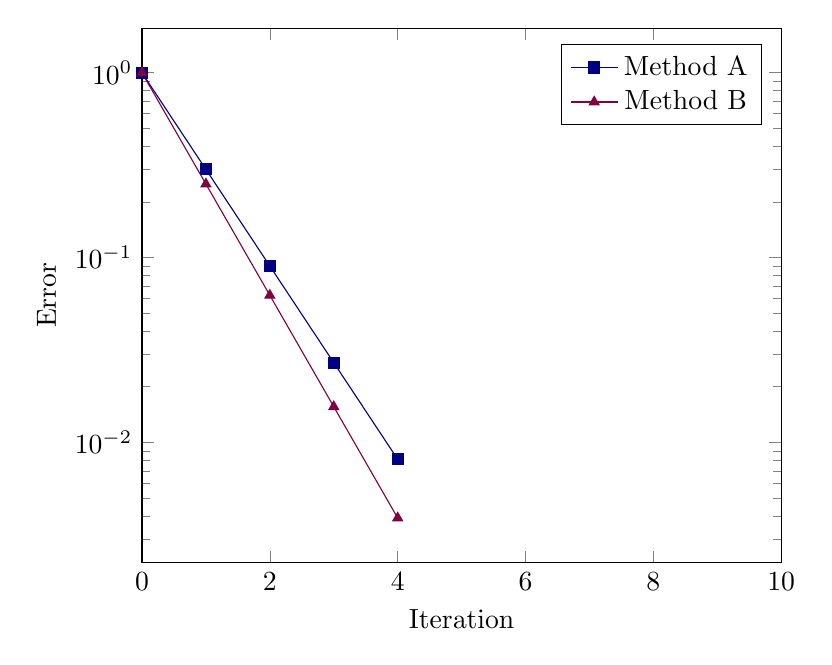
\begin{tikzpicture}
        \begin{axis}[
            width=0.8\linewidth,
            xlabel={Iteration},
            ylabel={Error},
            ymode=log,
            xmin=0, xmax=10,
            legend pos=north east
        ]
        \addplot[color=SomnusKeyword, mark=square*] coordinates {
            (0,1) (1,0.3) (2,0.09) (3,0.027) (4,0.0081)
        };
        \addlegendentry{Method A}
        \addplot[color=SomnusString, mark=triangle*] coordinates {
            (0,1) (1,0.25) (2,0.0625) (3,0.0156) (4,0.0039)
        };
        \addlegendentry{Method B}
        \end{axis}
    \end{tikzpicture}
    \caption{Convergence comparison between two methods.  Colours are
    reserved for plots and do not appear in the body text.}
    \label{fig:convergence}
\end{figure}

\section{Discussion}
Interpret your results, discuss limitations and relate your findings to
previous work.

\section{Conclusion}
Summarise the key insights and outline directions for future research.

% ----------------------------------------------------------------------
% Bibliography
\bibliographystyle{ieeetr}
% Create a file called references.bib alongside this template and add
% entries there.  Uncomment the next line to use it.
%\bibliography{references}

% ----------------------------------------------------------------------
\end{document}
